
    \begin{abstract_online}{Cold Adaptation of Cell Membrane of a Psychrotolerant Bacteria: Investigation using Molecular Dynamics Simulation}{%
        \underline{S. Erimban}, S. Daschakraborty}{%
        }{%
        Department of Chemistry, IIT Patna, Bihar 801106, India}
    Extensive and highly diversified areas of earth’s cold biosphere have a plethora of microbial assemblages with many mysteries regarding their survival strategies. These organisms survive and thrive in a variety of harsh conditions, which are not hospitable for life. These species are termed as extremophiles. Psychrophile is one such class that survives and thrives in some of the coldest regions of the earth’s biosphere. The adaptive strategies, which the psychrophiles acquire to survive against odds are called as cold adaptation. The cold adaptation of the cellular lipid membrane is the strategy taken by the cell to maintain the fluidity of the cell membrane, which is generally lost due to the fluid-to-gel phase transition of lipid membrane at low temperatures. The preservation of proper cell membrane fluidity is of paramount importance for the appropriate functioning of the cell. Modifications in the composition of different types of lipid molecules are a ubiquitous feature of cellular adaptation in psychrophiles. This is called as homeoviscous adaptation. Using coarse grained molecular dynamics simulation we have investigated such adaptation of a psychrotolerant bacteria’s cell membrane1. The key results of this work will be presented. \begin{center}  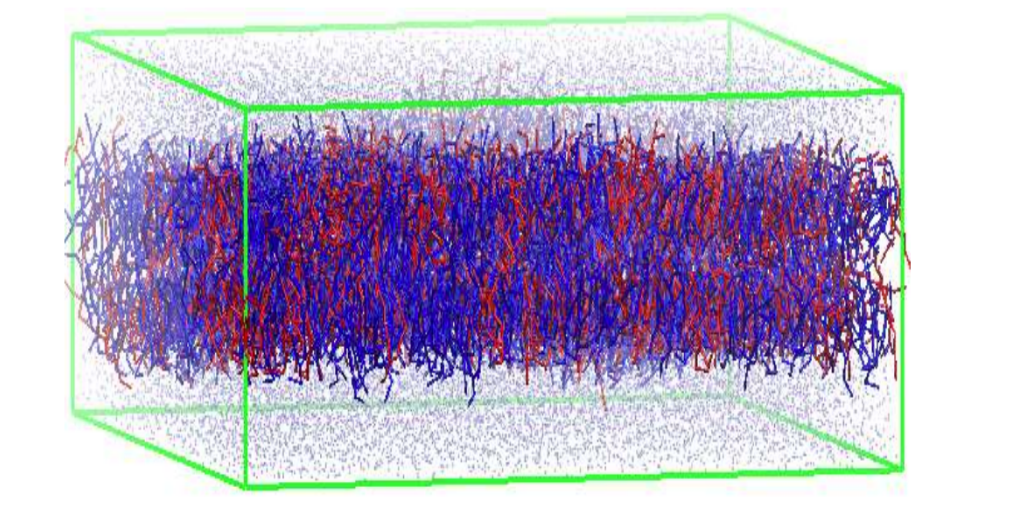
\includegraphics[width=0.9\linewidth]{abstracts/txt/figures/shakkira.png}  \caption{Snapshot of our simulated system modeled with the MARTINI Force field.}  \end{center}  
    
        \textbf{References} \newline{}[1] A. Singh, K. P. Krishnan, D. Prabaharan and R. K. Sinha, Journal of Basic Microbiology, 2017, 57, 770-780.
    \end{abstract_online}
    